\chapter{Use Case Diagram}

\section{Description}
The use case diagram (Figure \ref{fig:usecase}) shows the potential functions of our system for two actors: the Resident and the Visitor. Our use cases are listed in the following section by which actor is allowed the action and what preconditions, postconditions, and/or exceptions are there for the specific use case in our system.

\begin{figure}[h]
  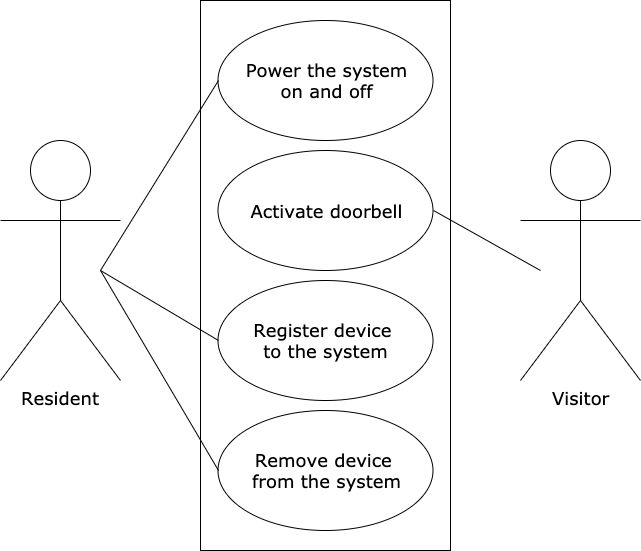
\includegraphics[width=0.8\textwidth]{UseCase-updated.png}
  \centering
  \caption{Use Case Diagram}
  \label{fig:usecase}
\end{figure}

\section{Functionality}

\subsection{Power System On and Off}
\begin{description}
\item [Actor:] Resident
\item [Goal:] Setting up system and personalizing it
\item [Postcondition:] System should safely shut off or turn on with previous settings
\end{description}
\subsection{Activate Doorbell}
\begin{description}
\item [Actor:] Visitor
\item [Goal]: Alert the Resident, that someone is at the door
\item [Precondition:] System is successfully activated with a device paired to it
\item [Postcondition:] Alert the Resident through their connected device(s)
\item [Exceptions:] Nothing happens if System is not active or device is disconnected
\end{description}
\subsection{Register Element to the System}
\begin{description}
\item [Actor:] Resident
\item [Goal:] Connect a device so Resident may be alerted of Visitor at door
\item [Precondition:]System is powered on successfully
\item [Postcondition:] Device is registered successfully to system and will be activated once prompted
\item [Exception:] Unsuccessful device registration and prompt user of error in pairing
\end{description}
\subsection{Remove Element from the System}
\begin{description}
\item [Actor:] Resident
\item [Goal:] Unregister device from the system when no longer using it
\item [Precondition:] System should be on
\item [Postcondition:] Device successfully unregistered
\end{description}